\pdfoutput=1
\pdfcompresslevel=9
\pdfinfo
{
    /Author (Autor)
    /Title (Tytul)
    /Subject (Tematyka)
    /Keywords (Slowa kluczowe)
}
%\documentclass[a4paper,polish,onecolumn,oneside,floatssmall,11pt,titleauthor,wide,openright]{mwrep}
%\usepackage[scale={0.7,0.8},paper=a4paper,twoside]{geometry}
\documentclass[a4paper,onecolumn,oneside,12pt,wide,floatssmall]{mwrep}
% \usepackage{polish}
\usepackage{amsmath}
\usepackage{amsfonts}
\usepackage{amssymb}
\usepackage{amsthm}
\usepackage{bookman}
\usepackage{geometry}
\usepackage[utf8x]{inputenc}
\usepackage[T1]{fontenc}
% \usepackage{t1enc}
% \usepackage[pdftex, bookmarks]{hyperref}
\usepackage[pdftex, bookmarks=false]{hyperref}
\def\url#1{{ \tt #1}}

\usepackage{listings}

% marginesy
\textwidth\paperwidth
\advance\textwidth -55mm
\oddsidemargin-0.9in
\advance\oddsidemargin 30mm
\evensidemargin-0.9in
\advance\evensidemargin 30mm
\topmargin -1in
\advance\topmargin 20mm
\setlength\textheight{48\baselineskip}
\addtolength\textheight{\topskip}
\marginparwidth15mm
\newgeometry{tmargin=2.5cm, bmargin=2.5cm, lmargin=3cm, rmargin=2.5cm}

\clubpenalty=10000 % to kara za sierotki
\widowpenalty=10000 % nie pozostawia wdów
\brokenpenalty=10000 % nie dzieli wyrazów pomiędzy stronami
\sloppy

\tolerance4500
\pretolerance250
\hfuzz=1.5pt
\hbadness1450

\usepackage[pdftex]{color,graphicx}
\usepackage[polish]{babel}
\usepackage[T1]{fontenc}
\usepackage{mathptmx}


% \textheight232mm
% \setlength{\textwidth}{\textwidth}
% \setlength{\oddsidemargin}{\evensidemargin}
% \setlength{\evensidemargin}{0.3cm}
\usepackage[sort, compress]{cite}

%\usepackage{multibib}
%\newcites{bk,st,doc,web}{Książki i~artykuły,Standardy i~zalecenia,Dokumentacja produktów,Publikacje i~serwisy internetowe}

\theoremstyle{definition}
\newtheorem{defn}{Definicja}[section]
\newtheorem{conj}{Teza}[section]
\newtheorem{conjmain}{Teza}
\newtheorem{exmp}{Przykład}[section]

\theoremstyle{plain}% default
\newtheorem{thm}{Twierdzenie}[section]
\newtheorem{lem}[thm]{Lemat}
\newtheorem{prop}[thm]{Hipoteza}
\newtheorem*{cor}{Wniosek}

\theoremstyle{remark}
\newtheorem*{rem}{Uwaga}
\newtheorem*{note}{Uwaga}
\newtheorem{case}{Przypadek}

\definecolor{ListingBackground}{rgb}{0.95,0.95,0.95}

\lstset{
        language=SQL,
    inputencoding=utf8x, 
    extendedchars=\true,
    literate={ą}{{\k{a}}}1
             {Ą}{{\k{A}}}1
             {ę}{{\k{e}}}1
             {Ę}{{\k{E}}}1
             {ó}{{\'o}}1
             {Ó}{{\'O}}1
             {ś}{{\'s}}1
             {Ś}{{\'S}}1
             {ł}{{\l{}}}1
             {Ł}{{\L{}}}1
             {ż}{{\.z}}1
             {Ż}{{\.Z}}1
             {ź}{{\'z}}1
             {Ź}{{\'Z}}1
             {ć}{{\'c}}1
             {Ć}{{\'C}}1
             {ń}{{\'n}}1
             {Ń}{{\'N}}1
}

\begin{document}

\renewcommand*\lstlistingname{Wydruk}
\renewcommand*\lstlistlistingname{Spis wydruków}

\pagenumbering{roman}
\renewcommand{\baselinestretch}{1.0}
\raggedbottom

\begin{titlepage}
    % Strona tytułowa
    \vbox to\textheight{\hyphenpenalty=10000
    \begin{center}
	\par\vspace{\smallskipamount}
	\vspace*{-4\baselineskip}{\fontsize{18}{18}\selectfont \textbf{PAŃSTWOWA WYŻSZA SZKOŁA ZAWODOWA}\\
\textbf{W NOWYM SĄCZU}\par}
	\vspace*{3\baselineskip}{\fontsize{18}{18}\selectfont INSTYTUT TECHNICZNY\par}
	\vspace*{7\baselineskip}{\fontsize{16}{16}\selectfont \textbf{PRACA DYPLOMOWA}\par}
	\vspace*{2\baselineskip}{\fontsize{16}{16}\selectfont SYSTEM GENEROWANIA RAPORTÓW W PROCESIE REKRUTACJI KANDYDATÓW NA STUDIA PROWADZONE W PWSZ W NOWYM SĄCZU.\par}

	\vspace*{10\baselineskip}
	
	%\hfill
	\begin{tabular}[b]{@{}l@{}}
	{\hspace*{5cm} \fontsize{14}{14}\selectfont \textbf{Autor:}} 
	{\fontsize{14}{14}\selectfont \textbf{Paweł Mysiński}}\\ \\
	{\hspace*{5cm} \fontsize{12}{12}\selectfont Kierunek:}
	{\fontsize{12}{12}\selectfont Informatyka}\\ \\
	{\hspace*{5cm} \fontsize{12}{12}\selectfont Nr albumu:}
	{\fontsize{12}{12}\selectfont 20747}
	\end{tabular}\par
	%\vspace*{4\baselineskip}
    \vspace*{6\baselineskip}{\fontsize{12}{12}\selectfont Promotor: dr inż. Antoni Ligęza\par}
    \vspace*{3\baselineskip}{\fontsize{14}{14}\selectfont \textbf{NOWY SĄCZ 2015}\par}
    \end{center}}

    \newpage\thispagestyle{empty}
	\mbox{}
	\newpage

\end{titlepage}

% ex: set tabstop=4 shiftwidth=4 softtabstop=4 noexpandtab fileformat=unix filetype=tex spelllang=pl,en spell:


\newpage
\pagenumbering{arabic}
\setcounter{page}{3}

\tableofcontents
% \addcontentsline{toc}{chapter}{{Przedmowa1}{vii}}{vii}

% \chapter*{Spis tablic, rysunków i~wydruków}
% \listoftables
% \listoffigures
% \lstlistoflistings

%\setlength{\baselineskip}{7mm}


\chapter{Wprowadzenie}

Listy, protokoły, decyzje oraz różnego typu dokumenty towarzyszące to nierozłączna część każdego procesu rekrutacji kandydatów na studia w uczelni wyższej. Sporządzenie wymienionych typów raportów, bez specjalizowanego oprogramowania, może prowadzić do powstania wielu problemów i związanych z nimi kosztów.  Trudno oczekiwać, aby uczelnia w momencie zamawiania takiego oprogramowania była w stanie przewidzieć jakiego rodzaju i w jakiej formie należy sporządzać w formie analogowej dokumentację procesu rekrutacyjnego. Stąd w większości uczelni, mimo obecności dedykowanego oprogramowania rekrutacyjnego, zmusza się powołane komisje rekrutacyjne do przygotowywania wielu dokumentów w sposób manualny, z wykorzystaniem podstawowego oprogramowania do składu tekstu. Takie postępowanie narażone jest na wiele pomyłek człowieka, przy ogromie zestawianych, w różnych formach, tych samych danych.  Dodać jeszcze należy, że w skład komisji rekrutacyjnych, co roku wchodzą różni pracownicy dydaktyczni uczelni (tak jest m.in. w przedmiotowej PWSZ w Nowym Sączu), którzy od początku muszą zorganizować swój warsztat pracy w sposób nieefektywny, ponieważ komisje byłe i obecne nie wymieniają między sobą żadnych informacji naprawczych poza jedną, że praca w komisji rekrutacyjnej to prawdziwa, nieoceniona udręka.


Z rozwiązaniem przedstawionego problemu może przyjść  informatyzacja tej części procesu rekrutacyjnego, która podlega corocznym zmianom. Pozwala ona w sposób niezależny od firmy dostarczającej oprogramowanie rekrutacyjne (oprogramowanie dostarczone jest wraz z bazą danych, z której można wydobyć w sposób autoryzowany określone dane), przygotować w placówce uczelni zestaw szablonowych dokumentów i połączyć je z danymi z systemu bazodanowego. W efekcie otrzymuje się wielostronicowe, uporządkowane zgodnie z przyjętą metodologią przekazywania raportów, pliki pdf, gotowe do wydruku na specjalizowanych urządzeniach drukująco\dywiz składająco\dywiz  kopertujących.


\section{Cel i zakres pracy}
Celem pracy jest opracowanie informatyczne systemu, który zapewni komisjom rekrutacyjnym możliwość przygotowania, drukowalnych wersji raportów  rekrutacyjnych, których brak w systemie rekrutacyjnym uczelni, lub sposób ich organizacji jest z grupy pseudoinformatyczno\dywiz usprawniających pracę.

Osiągnięcie postawionego celu, wymaga wykonania następujących zadań:
\begin{enumerate}
\item Wybór systemu do przygotowania szablonów raportów, wraz z systemem ich wizualnej prezentacji.
\item Wybór środowiska do utworzenia przenośnej wersji programu, który umożliwi wydobycie danych z baz uczeni i połączenie z szablonami w celu wygenerowania drukowanych wersji raportów w formacie pdf.
\item Utworzenie, aktualnych, szablonów dokumentów rekrutacyjnych w PWSZ w Nowym Sączu.
\item Zaimplementowanie programu oraz jego opis dokumentacyjny, umożliwiający w przyszłości wprowadzenie nowej funkcjonalności, jeżeli takie się pojawią.
\item Wygenerowanie danych testowych, symulujące rzeczywiste dane z bazy uczelnianej.
\item Przeprowadzenie testu działania systemu na wygenerowanych danych.
\item Przygotowanie dokumentacji oraz instrukcji obsługi systemu.
\item Obserwacja wykorzystania opracowanego systemu w rzeczywistym procesie rekrutacji w roku akademickim 2014, 2015, 2016 systemu w dedykowanej jednostce.
\end{enumerate}


\chapter{Uruchomienie oraz testowanie systemu}
Przed wdrożeniem programu do realnego systemu, program należy przetestować. Testy powinny być prowadzone na bazie danych która jest odwzorowaniem istniejącej już bazy, ponieważ idea testów jest taka, że po podmianie bazy danych na realną wszystko ma działać bez zmian. Jedyną różnicą może tylko zapis połączenia w pliku konfiguracyjnym. Do przeprowadzenia testów potrzebne więc będzie odtworzenie przyszłego środowiska, w którym będzie działać program, przygotować szablony dokumentów, które są wytwarzane w procesie rekrutacji oraz wygenerować dokumenty. Ostatnim już krokiem będzie sprawdzenie czy podczas tego procesu nie ma żadnych komplikacji oraz czy wygenerowane dokumenty nie zawierają błędów.
\section{Wstępne ustalenia}

Przed rozpoczęciem jakichkolwiek działań należy przygotować podstawowe rzeczy do rozpoczęcia testów.

\subsection{Specyfikacja maszyny do testów}
Testy przeprowadzone będą na komputerze o następującej specyfikacji:
\begin{lstlisting}
OS Name	Microsoft Windows 7 Ultimate
Version	6.1.7601 Service Pack 1 Build 7601
System Model	Z97-lstlisting
System Type	x64-based PC
Processor	Intel(R) Core(TM) i5-4590 CPU @ 3.30GHz,
3301 Mhz, 4 Core(s), 4 Logical Processor(s)
Installed Physical Memory (RAM)	8,00 GB
Total Physical Memory	7,86 GB
Available Physical Memory	3,99 GB
Total Virtual Memory	9,86 GB
Available Virtual Memory	3,75 GB
Page File Space	2,00 GB
\end{lstlisting}

Do działania programu \emph{DBRaportlatex} zainstalowana została JAVA w wersji:
\begin{lstlisting}
C:\Users\Pawlos>java -version
java version "1.8.0_60"
Java(TM) SE Runtime Environment (build 1.8.0_60-b27)
Java HotSpot(TM) 64-Bit Server VM (build 25.60-b23, mixed mode)
\end{lstlisting}

\subsection{Struktura katalogowa}

Do przejrzystego przechowywania wszystkich rzeczy potrzebnych w systemie rekrutacji, potrzebna będzie odpowiednia struktura katalogów. Do przechowywania potrzebne będą: \\
\begin{itemize}
\item program: \texttt{DBLatexRaport.jar}
\item plik konfiguracyjny: \texttt{dblatexraportconfig.bat}
\item środowisko kompilacji latex
\item szablony dokumentów 
\item plik bazy danych(tylko w testach)
\item pliki wynikowe
\item biblioteki potrzebne dla silnika bazy danych firebird w wersji embedded \\
\end{itemize}

Proponowana struktura więc może wyglądać następująco:

%\dirtree{%
 %.1 /.
 %.2 Firebird.
 %.2 output.
 %.2 template.
 %.2 texlive.
 %.2 DBLatexRaport.jar.
 %.2 dblatexraportconfig.bat.
 %.2 rekrutacja.fdb.
%}
\vspace{5mm}
Do katalogu \emph{texlive} przegrane zostało środowisko do kompilacji plików latex. W katalogu firebird są biblioteki tylko na czas testów do wersji embedded bazy danych. W katalogu \emph{template} zapisane zostaną szablony dokumentów.


\section{Generowanie przykładowych danych}

W celu przetestowania systemu generowania raportów w procesie rekrutacji kandydatów na studia potrzebne będą testowe dane w dokładnie tej samej strukturze, co w systemie rekrutacji, ze względu na fakt, iż w szablonach LaTeX znajdują się zapytania SQL do tabel w znajdujących się w bazie danych. 
W celu otrzymania tych danych potrzebne będzie:
\begin{enumerate}

\item	Utworzenie nowej bazy danych na silniku Firebird’a 
\item	Stworzenie struktury tabel odzwierciedlającą strukturę w systemie uczelnianym.
\item	Wygenerowanie wyczerpującej potrzeby testu ilości testowych danych osobowych.
\item	Uzupełnienie tabel danymi, które zostały wygenerowane wcześniej oraz dodanie do nich dodatkowych, jednocześnie losowych, informacji na temat procesu rekrutacji.
\vspace{5mm}
\end{enumerate}
Po wykonaniu tych kroków, powinna powstać baza danych do której bez problem program połączy się i uzyska z niej potrzebne dane dokładnie w ten sam sposób jak z realnej bazy danych.

\subsection{ Tworzenie bazy danych }

Do stworzenia pliku bazy danych na silniku firebird’a posłużyć się można narzędziem dostępnym w katalogu bin zainstalowanego serwera firebird.  Narzędzie to pozwala z linii komend tworzyć i łączyć się z bazami danych. W tym przypadku użyta zostanie komenda \texttt{CREATE DATABASE}
\begin{lstlisting}
C:\Program Files\Firebird\bin>isql
SQL>CREATE DATABASE 'D:\test systemu\rekrutacja.fdb'
CON>user 'SYSDBA' password 'masterkey';
\end{lstlisting}
Po wykonaniu tego polecenia zostanie utworzona baza danych. Takie same dane należy teraz wpisać do pliku konfiguracyjnego programu czyli \texttt{DBLatexRaport.bat} aby program mógł się połączyć z tą bazą:
\begin{lstlisting}
dbengine=firebirdsql
hostname=//localhost
port=3050
dbpath=D:\test systemu\rekrutacja.fdb
user=SYSDBA
password= masterkey
\end{lstlisting}
\subsection{ Stworzenie struktury bazy}

Dotychczasowy system wykorzystywał tabelę (widok) która była generowana dynamicznie i która zawiera wszystkich kandydatów w rekrutacji. Zawiera ona wszystkie dane potrzebne do wytworzenia dokumentów. Jeden rekord to jeden student ze wszystkimi informacjami na jego temat. Dodatkowo jeszcze potrzebna jest tabela z informacjami na temat rekrutacji, takimi jak na przykład nazwisko i imię przewodniczącego komisji, czy data wydania decyzji przyjęcia studenta. Z tych tabel będą pobierane informacje, natomiast do wygenerowania danych potrzebne będą dwie dodatkowe tymczasowe tabele.
Tabela główna z kandydatami(zapis SQL):
\begin{lstlisting}
CREATE TABLE KANDYDAT_ALIGEZA (
    STUD_ID                        INTEGER NOT NULL,
    OSOBA_ID                       INTEGER NOT NULL,
    STUD_NRTECZKI                  INTEGER,
    NAZWISKO                       VARCHAR(100),
    IMIE                           VARCHAR(100),
    NAZWISKOIMIONA                 VARCHAR(200),
    ADR_ULICA_MIEJSCOWOSC_NR_DOMU  VARCHAR(200),
    ADR_KOD_POCZTOWY_POCZTA        VARCHAR(100),
    STUDIA_NAZWA                   VARCHAR(100),
    STUD_ILPUNKTOW                 INTEGER,
    STUD_ILPUNKTOWKREM             INTEGER,
    TOKNAUKI_NAZWATOKU             VARCHAR(200),
    KIERUNEK                       VARCHAR(100),
    SPEC_ID                        INTEGER,
    DATAPRZYJECIAPODANIA           DATE,
    TOKNAUKI_ID                    INTEGER,
    OSOBA_PESEL                    VARCHAR(50),
    KIERUNEK_MY                    VARCHAR(200),
    FORMA_STUDIOW_MY               VARCHAR(200),
    STOPIEN_STUDIOW_MY             VARCHAR(100),
    KIERUNEK_FORMA_SKROT_MY        VARCHAR(100),
    NR_DECYZJI                     VARCHAR(100),
    CZY_PRZYJETY                   INTEGER,
    DATA_DECYZJI                   DATE,
    ILE_PUNKTOW                    INTEGER,
    PANPANI                        CHAR(1)
);
\end{lstlisting}
Tabela z dodatkowymi informacjami(wartości przypisane są do kluczy tekstowych, jest to tablica asocjacyjna):
\begin{lstlisting}
CREATE TABLE SETUP_ALIGEZA (
    KLUCZ    VARCHAR(50) NOT NULL,
    WARTOSC  VARCHAR(100)
);
\end{lstlisting}
Tymczasowa tabela do zaimportowania listy imion i nazwisk oraz losowych peseli.
\begin{lstlisting}
CREATE TABLE DANE (
    IMIE_NAZ  VARCHAR(200),
    ADRES     VARCHAR(200),
    PESEL     VARCHAR(50),
    NAZWISKO  VARCHAR(100),
    IMIE      VARCHAR(100)
);
\end{lstlisting}
Tymczasowa tabela do procedury losowego uzupełniania informacji o rekrucie o kierunku jaki wybrał.
\begin{lstlisting}
CREATE TABLE TOKNAUKI_ALIGEZA (
    TOKNAUKI_ID              INTEGER NOT NULL,
    KIERUNEK_MY              VARCHAR(50),
    FORMA_STUDIOW_MY         VARCHAR(50),
    STOPIEN_STUDIOW_MY       VARCHAR(50),
    KIERUNEK_FORMA_SKROT_MY  VARCHAR(10),
    LICZBA_MIEJSC            SMALLINT,
    DATA_DECYZJI_OD          TIMESTAMP,
    DATA_DECYZJI_DO          TIMESTAMP,
    KOD_IKR                  VARCHAR(3)
);
\end{lstlisting}
\subsection{ Generowanie testowych danych osobowych}

Do wygenerowania kandydatów potrzebne jest imię, nazwisko oraz adres. Takie dane dostępne są w książkach telefonicznych. Posługując się jedną z nich stworzony został plik \emph{CSV} o separatorze „;” zawierający po kolei imię z nazwiskiem, adres, pesel, nazwisko oraz imię. Pesel został dodany do każdej osoby jako losowy ciąg cyfr spełniający walidację peselu. Ze względu na fakt iż pesel został wygenerowany losowo,  w wygenerowanych dokumentach nie będzie poprawnie przypisana płeć do imienia. Dlatego tylko do testów ustawione zostanie 5 pierwszych kandydatów jako płeć żeńska, a cała reszta męska.\\
Struktura pliku:
\begin{lstlisting}
 Abram Andrzej; Lwowska 116;88071640299;Abram;Andrzej
 Abram Halina; Ludwika Zamenhofa 2;86111210691;Abram;Halina
...

\end{lstlisting}

Tak sformatowany plik \emph{CSV},  łatwo zaimportować do bazy danych do tabeli \texttt{dane} ze względu na identyczną kolejność danych w kolumnach. Do importu wykorzystana została funkcja programu \emph{IBExpert}, \texttt{import data}. Jedna linijka w pliku zostaje zaimportowana jako jeden rekord, w którym każde pole po kolei odpowiada wartościom między średnikami. Zaimportowanych w ten sposób zostało 10001 rekordów (osób) do tabeli \texttt{dane} do dalszych manipulacji, co całkowicie wyczerpuje ilość kandydatów potrzebnych do testów. Ze statystyk wynika, że na uczelni średnio na rekrutacje przypada około trzystu kandydatów.

\subsection{Generowanie kandydatów na studentów}

Kolejnym krokiem jest uzupełnienie tabeli z tokami studiów. W testach dodanych zostało 8 przykładowych toków nauki. 

\begin{lstlisting}
1 Informatyka	niestacjonarne	pierwszego stopnia	INF-n				
2 Mechatronika	niestacjonarne	pierwszego stopnia	MT-n				
3 Mechatronika	stacjonarne	pierwszego stopnia	MT-s				
...
\end{lstlisting}
Uzupełnienia wymaga także tabela z dodatkowymi informacjami \texttt{setup\_aligeza} przykładowymi danymi:
\begin{lstlisting}
dataWydaniaDecyzji	09.10.2015
miejsceWydaniaDecyzji	Nowy Sącz
przewodniczacyIKR	mgr inż. Sławomir Jurkowski
rokAkademicki	2015/2016
czyUwzglednicDateWydaniaDecyzji	N
...

\end{lstlisting}

Mając już to wszystko potrzebna jest procedura, która utworzy listę kandydatów z tych wszystkich danych. 

\begin{lstlisting}
create procedure GENERUJ
returns (
    TESTCHAR varchar(50),
    TEST integer)
as
declare variable IMIE varchar(100);
declare variable NAZ varchar(100);
declare variable IMIENAZ varchar(200);
declare variable ADRES varchar(200);
declare variable PESEL varchar(50);
declare variable LICZNIK integer;
declare variable STOPIEN varchar(50);
declare variable KIERUNEK varchar(50);
declare variable FORMA varchar(50);
declare variable SKROT varchar(10);
declare variable RANDINT integer;
declare variable PUNKTY integer;
declare variable CZY_PRZYJETY integer;
declare variable DATA_DEC varchar(100);
begin
licznik = 1;
for select * from dane into
:imienaz,:adres,:pesel,:naz,:imie
do
begin
randint = CAST(round(rand()*7+1) as INTEGER);
punkty = CAST(round(rand()*500) as INTEGER);
if(punkty > 250) then czy_przyjety = 1;
if(punkty <= 250) then czy_przyjety = 2;

select kierunek_my,forma_studiow_my,stopien_studiow_my,
kierunek_forma_skrot_my
FROM toknauki_aligeza where toknauki_id = :randint
INTO :kierunek,:forma,:stopien,:skrot;

select wartosc FROM setup_aligeza 
WHERE klucz='dataWydaniaDecyzji'
INTO :data_dec;

INSERT INTO kandydat_aligeza (stud_id,osoba_id,stud_nrteczki,nazwisko,imie,
	nazwiskoimiona,adr_ulica_miejscowosc_nr_domu,adr_kod_pocztowy_poczta,
	osoba_pesel,panpani, studia_nazwa,toknauki_nazwatoku,kierunek, 
	kierunek_my,forma_studiow_my,stopien_studiow_my,
	kierunek_forma_skrot_my,    stud_ilpunktow,stud_ilpunktowkrem,
	ile_punktow,czy_przyjety,data_decyzji,nr_decyzji,dataprzyjeciapodania)
VALUES (:licznik,:licznik,cast(round(rand()*200+1) as integer),
	:naz,:imie,:imienaz,:adres, cast( 'Nowy Sacz 33-300' as varchar(100)),
	:pesel,cast( 'M' as char(1)),    :forma,:kierunek || 
	' N inz. 3.50 2015/2016 zimowy',:kierunek,:kierunek,:forma,
	:stopien,:skrot,    :punkty,:punkty,:punkty,:czy_przyjety,
	cast(:data_dec as DATE),'328/2015','2015-08-14');

licznik = :licznik + 1;
end
test = :licznik;
suspend;
end
\end{lstlisting}
Powyższa procedura z jednej osoby z tabeli \texttt{dane} tworzy jednego kandydata, losując mu tok nauki, ilość punktów oraz czy zostanie przyjęty lub nie. Dodawane są także pewne stałe wartości, podobne do tych w oryginalnej bazie danych, które nie wymagają uzmiennienia. Procedura ta, po jednorazowym wywołaniu, wygenerowała 10001 rekordów w tabeli \texttt{kandydat\_aligeza}. Daje to wystarczającą ilość testowych kandydatów do przeprowadzenia testów. Baza danych z przeprowadzonych testów znajduje się w załączniku.

\section{Dodanie zapytań SQL do szablonów}

Stworzone szablony w poprzednim rozdziale nie zawierają zapytań, które odzwierciedlały by wyselekcjonowanie danych z istniejącej struktury bazy. Zawierają tylko sztywne dane testujące środowiska LaTeX'owe. Aby szablony podczas procesu tworzenia dokumentów zostały uzupełnione poprawnymi danymi potrzeba je uzupełnić o odpowiednia zapytania SQL w odpowiedniej formie tak aby parser zawarty w programie był wstanie je znaleźć i wykonać.
\par 
Potrzebnych jest 9 zapytań, za pomocą których wyciągnięte zostaną dane do szablonów. Poniżej opisane zostały każde z zapytań oraz dla każdego przykład danych jakie zostaną wyselekcjonowane z bazy przez to zapytanie. Ta sekcja skupia się tylko i wyłącznie na uzyskaniu potrzebnych danych do środowisk LaTeX'a, a nie na tym jak one zostaną wykorzystane. Dokładny opis jak wygląda wykorzystanie takiego zapisu znajduje się w rozdziale \ref{ch:szablonyraportowwsystemielatex}. Dodać jeszcze należy ze poniższe zapytania znajdują się pod koniec każdego szablonu, zaraz po zdefiniowaniu środowisk. Takie umiejscowienie tych zapytań sprawi, że dane zostaną uzupełnione zaraz pod tymi zapytaniami.
\par 
\subsubsection*{Szablon z ustawieniami - aaasetup.tex}
Pierwsze zapytanie które zostanie omówione jest to  zapytanie o podstawowe parametry, informacje na temat rekrutacji. Znajduje się ono w pliku \emph{aaasetup.tex}. Plik posiada trzy litery "a" w nazwie, ponieważ program parsujący, otwiera pliki alfabetycznie a zapytanie to, musi zostać wykonane jako pierwsze.  Poniżej mamy przykład danych do zapisania:
 \begin{lstlisting}
\parametrRekrutacyjny{dataWydaniaDecyzji}{09.10.2015}
\parametrRekrutacyjny{miejsceWydaniaDecyzji}{Nowy Sącz}
\parametrRekrutacyjny{rokAkademicki}{2015/2016}
...
\end{lstlisting}
Aby uzyskać takie dane, potrzeba będzie pobrać wszystkie rekordy z tabeli \texttt{setup\_aligeza} (struktura tabeli znajduje się w poprzedniej sekcji) klucz oraz wartość. Zapytanie nie będzie więc zbyt skomplikowane:
 \begin{lstlisting}
SELECT klucz,wartosc FROM setup_aligeza
\end{lstlisting}
Po wywołaniu go, otrzymamy potrzebne nam dane. Jednak aby program parsujący był wstanie znaleźć takie zapytanie w szablonie potrzeba je obudować w odpowiednią konstrukcję, która będzie odpowiadać wyrażeniu regularnemu zapisanemu w parserze. Należy także wpisać nazwę środowiska w odpowiednie miejsce między znakami @@. Dodatkowo należy jeszcze postarać się aby kompilator LaTeX'a zignorował ten zapis i go nie wyświetlał. Do tego celu zastosowana została komenda \texttt{iffalse}.
 \begin{lstlisting}
\iffalse@@parametrRekrutacyjny@@
SELECT klucz,wartosc FROM setup_aligeza
@END@\fi
\end{lstlisting}
\subsubsection*{Szablon protokołu przekazania -  protokolprzekazania.tex}
Następnie zapytanie zawarte w pliku \emph{protokolprzekazania.tex}. Występuje tu nowy problem otworzenia środowiska na początku oraz zamknięcia na końcu. Pokazane jest to na przykładowych danych poniżej:
 \begin{lstlisting}
\protokolprzekazaniaA{1}
\protokolprzekazania{Informatyka ---
 niestacjonarne STUDIA pierwszego stopnia}{1455}
\protokolprzekazania{Informatyka ---
 stacjonarne STUDIA pierwszego stopnia}{729}
\protokolprzekazania{Mechatronika ---
 niestacjonarne STUDIA pierwszego stopnia}{1447}
...
\endprotokolprzekazaniaA        
\end{lstlisting}
\par
Pomijając na razie otwarcie środowiska \texttt{protokolprzekazaniaA\{1\} }oraz zamkniecie \texttt{endprotokolprzekazaniaA}, w zapytaniu potrzebne jest wyświetlić każdy tok nauczania oraz zagregowaną liczbę kandydatów na tym toku. Do agregacji użyte zostanie polecenie \texttt{group} na polu tok by móc otrzymać liczbę kandydatów używając funkcji count(*). Dodatkowo potrzeba także wybrać kandydatów, posiadających daną datę decyzji. Do tego posłuży podzapytanie, które pobierze datę decyzji z aktualnej rekrutacji i porówna ją z datą decyzji dla danego kandydata. 
 \begin{lstlisting}
SELECT  k.kierunek_my||' --- '||k.forma_studiow_my||
' STUDIA '||k.stopien_studiow_my AS tok, count(*) AS ile
FROM kandydat_aligeza k
WHERE  k.data_decyzji=(SELECT wartosc FROM
 setup_aligeza WHERE klucz='dataWydaniaDecyzji') 
GROUP BY tok
\end{lstlisting}
\par
Takie zapytanie wyświetli dane pomiędzy tymi pominiętymi dotychczas komendami. 
Rozwiązaniem wyświetlenia tych komend jest funkcja programu uzupełniającego szablony, a dokładnie funkcja grupowania. Dokładny opis tej funkcji znajduje się w rozdziale \ref{ch:szablonyraportowwsystemielatex}. Do zapytania dodamy jako pierwsze pole wartość 1, a następnie użyta zostanie funkcja grupowania po 1 polu wewnątrz szablonu:
 \begin{lstlisting}
\iffalse @@protokolprzekazania@1@@
SELECT 1 AS n,k.kierunek_my||' --- '||
k.forma_studiow_my||' STUDIA '||
k.stopien_studiow_my AS tok, count(*) AS ile
FROM kandydat_aligeza k
WHERE  k.data_decyzji=(SELECT wartosc FROM
 setup_aligeza WHERE klucz='dataWydaniaDecyzji') 
GROUP BY tok
@END@\fi
\end{lstlisting}

\subsubsection*{Szablon z nadrukami na koperty- pocztex.tex}
Dla szablonu 'pocztex.tex' potrzebna jest prosta lista z adresami każdego kandydata z danej rekrutacji:


 \begin{lstlisting}
\iffalse@@pocztex@@
SELECT ka.nazwiskoimiona,
       ka.adr_ulica_miejscowosc_nr_domu,
	   ka.adr_kod_pocztowy_poczta,
	   ka.stud_nrteczki||' '||ka.kierunek_forma_skrot_my||' '||ka.stud_id	   
FROM kandydat_aligeza ka 
WHERE  ka.data_decyzji=
(select wartosc from setup_aligeza 
where klucz='dataWydaniaDecyzji')
ORDER BY ka.kierunek_forma_skrot_my, ka.nazwiskoimiona
@END@\fi
\end{lstlisting}

\subsubsection*{Szablon z listami kandydatów do sekretariatu - listasekretariat.tex}
W kolejnym szablonie \emph{listasekretariat.tex} potrzebne jest utworzenie list kandydatów dla każdego toku nauki. Przez tok nauki rozumie się każdą kombinację kierunku, formy oraz stopnia studiów. W szablonie zostało to rozwiązane tak, że każda lista otwiera się poprzez wywołanie komendy \texttt{listarsekretariatA} z trzema parametrami, którymi są właśnie kierunek, forma oraz stopień studiów. Na przykładowych danych wygląda to następująco:
 \begin{lstlisting}
\listarsekretariatA{drugiego stopnia}{Informatyka}{stacjonarne}
\listarsekretariat{ Ablewicz Monika}{39}
\listarsekretariat{ Abram Halina}{69}
...
\endlistarsekretariatA
\listarsekretariatA{drugiego stopnia}{Mechatronika}{stacjonarne}
\listarsekretariat{ Adamek Danuta}{141}
\listarsekretariat{ Adamek Urszula}{35}
\listarsekretariat{ Adamik Zbigniew}{95}
...
\endlistarsekretariatA
...
\end{lstlisting}

W zapytaniu więc potrzebne będzie wybrać wszystkich kandydatów z datą decyzji aktualnej rekrutacji, a następnie wyświetlić kierunek, formę, stopień studiów, imię, nazwisko oraz numer teczki. W zapytaniu także potrzebne będzie sortowanie po polach, które będą grupowane w programie uzupełniającym szablon. W zapytaniu SQL zastosowane zostanie polecenie \texttt{ORDER BY} na grupowanych polach. Ostatecznie w odpowiednim miejscu pomiędzy nazwą a zapytaniem wpisana zostanie liczba "3", oznaczająca polecenie aby dane grupowane były po 3 pierwszych polach:
 \begin{lstlisting}
\iffalse@@listarsekretariat@3@@
SELECT stopien_studiow_my,kierunek_my,forma_studiow_my,
       nazwiskoimiona,stud_nrteczki
FROM kandydat_aligeza
WHERE data_decyzji=
(select wartosc from setup_aligeza
 where klucz='dataWydaniaDecyzji')
ORDER BY kierunek_forma_skrot_my, nazwiskoimiona
@END@\fi
\end{lstlisting}

\subsubsection*{Szablony z listami listaprzyjetych.tex, listanieprzyjetych.tex, listawysylkowa.tex, listarankingowa.tex}
W szablonach znajdują się jeszcze 4 kolejne podobne listy: przyjętych, nieprzyjętych, wysyłkowa oraz rankingowa. Zasada utworzenia zapytań do tych list jest identyczna jak w liście do sekretariatu. Różnią się one jedynie pewnymi warunkami wewnątrz zapytań SQL czy też polami po których będą sortowane dane.

\par Lista przyjętych:
 \begin{lstlisting}
\iffalse@@listaprzyjetych@3@@
SELECT stopien_studiow_my,kierunek_my,forma_studiow_my,
       nazwiskoimiona 
FROM kandydat_aligeza 
WHERE czy_przyjety=1 and
     data_decyzji=
     (SELECT wartosc FROM setup_aligeza 
     WHERE klucz='dataWydaniaDecyzji')
ORDER BY kierunek_forma_skrot_my,
         nazwiskoimiona
@END@\fi
\end{lstlisting}
\par Lista nieprzyjętych:
 \begin{lstlisting}
\iffalse@@listaprzyjetych@3@@
SELECT stopien_studiow_my,kierunek_my,forma_studiow_my,
       nazwiskoimiona 
FROM kandydat_aligeza 
WHERE czy_przyjety=2 and
     data_decyzji=(SELECT wartosc FROM setup_aligeza 
     WHERE klucz='dataWydaniaDecyzji')
ORDER BY kierunek_forma_skrot_my,
         nazwiskoimiona
@END@\fi
\end{lstlisting}
\par Lista wysyłkowa:
 \begin{lstlisting}
\iffalse @@listawysylkowa@3@@
SELECT stopien_studiow_my,kierunek_my,forma_studiow_my,
      nazwiskoimiona, adr_ulica_miejscowosc_nr_domu||'; '||
       ADR_KOD_POCZTOWY_POCZTA
FROM kandydat_aligeza 
WHERE data_decyzji=(select wartosc from setup_aligeza 
where klucz='dataWydaniaDecyzji')
ORDER BY kierunek_forma_skrot_my, nazwiskoimiona
@END@\fi
\end{lstlisting}
\par Lista rankingowa:
 \begin{lstlisting}
\iffalse@@listarankingowa@3@@
SELECT stopien_studiow_my,kierunek_my,forma_studiow_my,
       nazwiskoimiona,STUD_ILPUNKTOW
FROM kandydat_aligeza
WHERE  data_decyzji=(select wartosc from setup_aligeza 
where klucz='dataWydaniaDecyzji')
ORDER BY kierunek_forma_skrot_my, STUD_ILPUNKTOW desc
@END@\fi
\end{lstlisting}
\par 
\subsubsection*{Szablon z decyzją odnośnie przyjęcia kandydata - decyzja.tex}
W ostatnim szablonie wystąpił problem ilości parametrów jakie trzeba przekazać do poprawnego działania szablonu. W LaTeX'ie można stworzyć środowisko o maksymalnie 9 parametrach, natomiast w szablonie \emph{decyzja.tex} dla każdego kandydata potrzeba 12 różnych informacji. Rozwiązaniem tego problemu także było grupowanie przez program uzupełniania raportów. Funkcja grupująca wycina 3 pierwsze pola i wstawia je do nowego środowiska. Dodatkowo w zapytaniu SQL wyświetlanie daty musi posiadać dodatkowe 0 przy datach typu 01.02.2015 gdzie właśnie liczby dni lub miesięcy są mniejsze od 10:
 \begin{lstlisting}
\iffalse@@decyzja@3@@
SELECT ka.stopien_studiow_my,ka.kierunek_my,ka.forma_studiow_my,
	ka.stud_ilpunktow,ka.nr_decyzji,ka.nazwiskoimiona,ka.adr_ulica_miejscowosc_nr_domu,
	ka.adr_kod_pocztowy_poczta,ka.stud_nrteczki||' '||ka.kierunek_forma_skrot_my||
	' '||ka.stud_id,czy_przyjety,extract(day from ka.dataprzyjeciapodania)||'.'||
	substring(100+extract(month from ka.dataprzyjeciapodania) from 2 for 2)||'.'||
	extract(year from ka.dataprzyjeciapodania), panpani
FROM kandydat_aligeza ka 
WHERE  ka.data_decyzji=(select wartosc from setup_aligeza 
where klucz='dataWydaniaDecyzji')
ORDER BY ka.kierunek_forma_skrot_my, ka.nazwiskoimiona
@END@\fi
\end{lstlisting}

\section{Konfiguracja programu}

W głównym katalogu znajduje się plik konfiguracyjny programu o nazwie  \emph{dblatexraportconfig.bat}. Plik ten jest jednocześnie plikiem wsadowym oraz zawiera konfiguracje programu \emph{DBRaportlatex.jar}. Część kodu batch uruchamia program DBraportlatex razem z odpowiednimi parametrami do uruchomienia \emph{embedded firebird}:
 \begin{lstlisting}
@echo off
java -Djava.library.path=.\firebird -jar dbraportlatex.jar
pause
exit
\end{lstlisting}

Następnie od linijki zawierającej \texttt{\#dbLatexRaportConfig} zaczynają się zmienne konfiguracyjne:
  \begin{itemize}
  \item Ścieżka do szablonów LaTeX
   \begin{lstlisting}
templatepath=template/
  \end{lstlisting}
  \item Ścieżka do uzupełnionych szablonów LaTeX oraz skompilowanego pliku PDF
  \begin{lstlisting}
output=output/
 \end{lstlisting}
  \item Kodowanie szablonów LaTeX
   \begin{lstlisting}
encodingtex=UTF-8
  \end{lstlisting}
   \item Konfiguracja połączenia z bazą danych
    \begin{lstlisting}
dbengine=firebirdsql
hostname=embedded
dbpath=rekrutacja.fdb
user=SYSDBA
password=
dbencoding=WIN1250
   \end{lstlisting}
  \item Ścieżka do komilatora LaTeX
   \begin{lstlisting}
pdflatexpath=texlive\2010min\bin\win32\pdflatex.exe
  \end{lstlisting}
    \item Lista plików do kompilacji
 \begin{lstlisting}
pdfcompilemainfile=main.tex,main.tex
\end{lstlisting}
\end{itemize}
\section{Przebieg testu}

W bazie danych znajduje się 10001 kandydatów. Należy spodziewać się tyle samo wygenerowanych na listach.  Program został uruchomiony z pliku wsadowego \emph{dblatexraportconfig.bat}. Poniżej znajduje się wydruk z konsoli po uruchomieniu programu z krótkimi opisami poszczególnych procesów:

\begin{enumerate}
\item Ładowanie pliku konfiguracyjnego przez program:
\begin{lstlisting}
Config loaded: dblatexraportconfig.bat
pattern=
templatepath=template/
output=output/
encodingtex=UTF-8
dbengine=firebirdsql
hostname=embedded
dbpath=rekrutacja.fdb
user=SYSDBA
password=*********
dbencoding=WIN1250
pdflatexpath=texlive\2010min\bin\win32\pdflatex.exe
pdfcompilemainfile=main.tex,main.tex
 \end{lstlisting}
 
 \item Połączenie z bazą danych:
\begin{lstlisting}
Connection to database: OK
 \end{lstlisting}
 
  \item Ładowanie szablonów do pamięci:
\begin{lstlisting}
Loaded file: template\aaasetup.tex
Loaded file: template\decyzja.tex
Loaded file: template\listanieprzyjetych.tex
Loaded file: template\listaprzyjetych.tex
Loaded file: template\listarankingowa.tex
Loaded file: template\listarsekretariat.tex
Loaded file: template\listawysylkowa.tex
Loaded file: template\main.tex
Loaded file: template\pocztex.tex
Loaded file: template\protokolprzekazania.tex
 \end{lstlisting}
 
   \item Wywoływanie zapytań SQL oraz uzupełnianie szablonów:
 \begin{lstlisting}
aaasetup.tex - processing SQL statements
no returns SQL1
9 records SQL2

decyzja.tex - processing SQL statements
10001 records SQL1

listanieprzyjetych.tex - processing SQL statements
5051 records SQL1

listaprzyjetych.tex - processing SQL statements
4950 records SQL1

listarankingowa.tex - processing SQL statements
10001 records SQL1

listarsekretariat.tex - processing SQL statements
10001 records SQL1

listawysylkowa.tex - processing SQL statements
10001 records SQL1

main.tex - processing SQL statements

pocztex.tex - processing SQL statements
10001 records SQL1

protokolprzekazania.tex - processing SQL statements
8 records SQL1

 \end{lstlisting}
 
   \item Zapisywanie uzupełnionych szablonów do katalogu wynikowego:
 \begin{lstlisting}
Saved to file: output/aaasetup.tex
Saved to file: output/decyzja.tex
Saved to file: output/listanieprzyjetych.tex
Saved to file: output/listaprzyjetych.tex
Saved to file: output/listarankingowa.tex
Saved to file: output/listarsekretariat.tex
Saved to file: output/listawysylkowa.tex
Saved to file: output/main.tex
Saved to file: output/pocztex.tex
Saved to file: output/protokolprzekazania.tex

 \end{lstlisting}
 
   \item Wywoływanie kompilatora LaTeX dla głównego pliku \emph{main.tex}, co spowoduje skompilowanie wszystkich szablonów:
 \begin{lstlisting}
Executing shell command:
cmd /c start texlive\2010min\bin\win32\pdflatex.exe
 --output-directory=output/ output/main.tex
Executing shell command:
cmd /c start texlive\2010min\bin\win32\pdflatex.exe
 --output-directory=output/ output/main.tex

WORK DONE!!!

Directory pdf results output: output/
 \end{lstlisting}
\end{enumerate}
Program wykonał się bez żadnych błędów i wykonał swoje zadanie. Uzupełnienie szablonów trwało poniżej 1 sekundy, natomiast podwójna kompilacja wszystkich szablonów około jednej minuty, co spełnia założenia projektu. 

\section{Wyniki testu}
Wszystkie szablony zostały uzupełnione poprawnie danymi z bazy danych oraz kompilacja systemu LaTeX przebiegła bezproblemowo. Na rysunku \ref{fig:test} przedstawione zostały wybrane strony z wygenerowanych dokumentów. W pliku wynikowym PDF ze wszystkimi dokumentami gotowymi do druku wszystko jest zgodnie z oczekiwaniami. Wygenerowany plik PDF z testów dołączony jest w załączniku.

\begin{figure}[h]
    \centering
    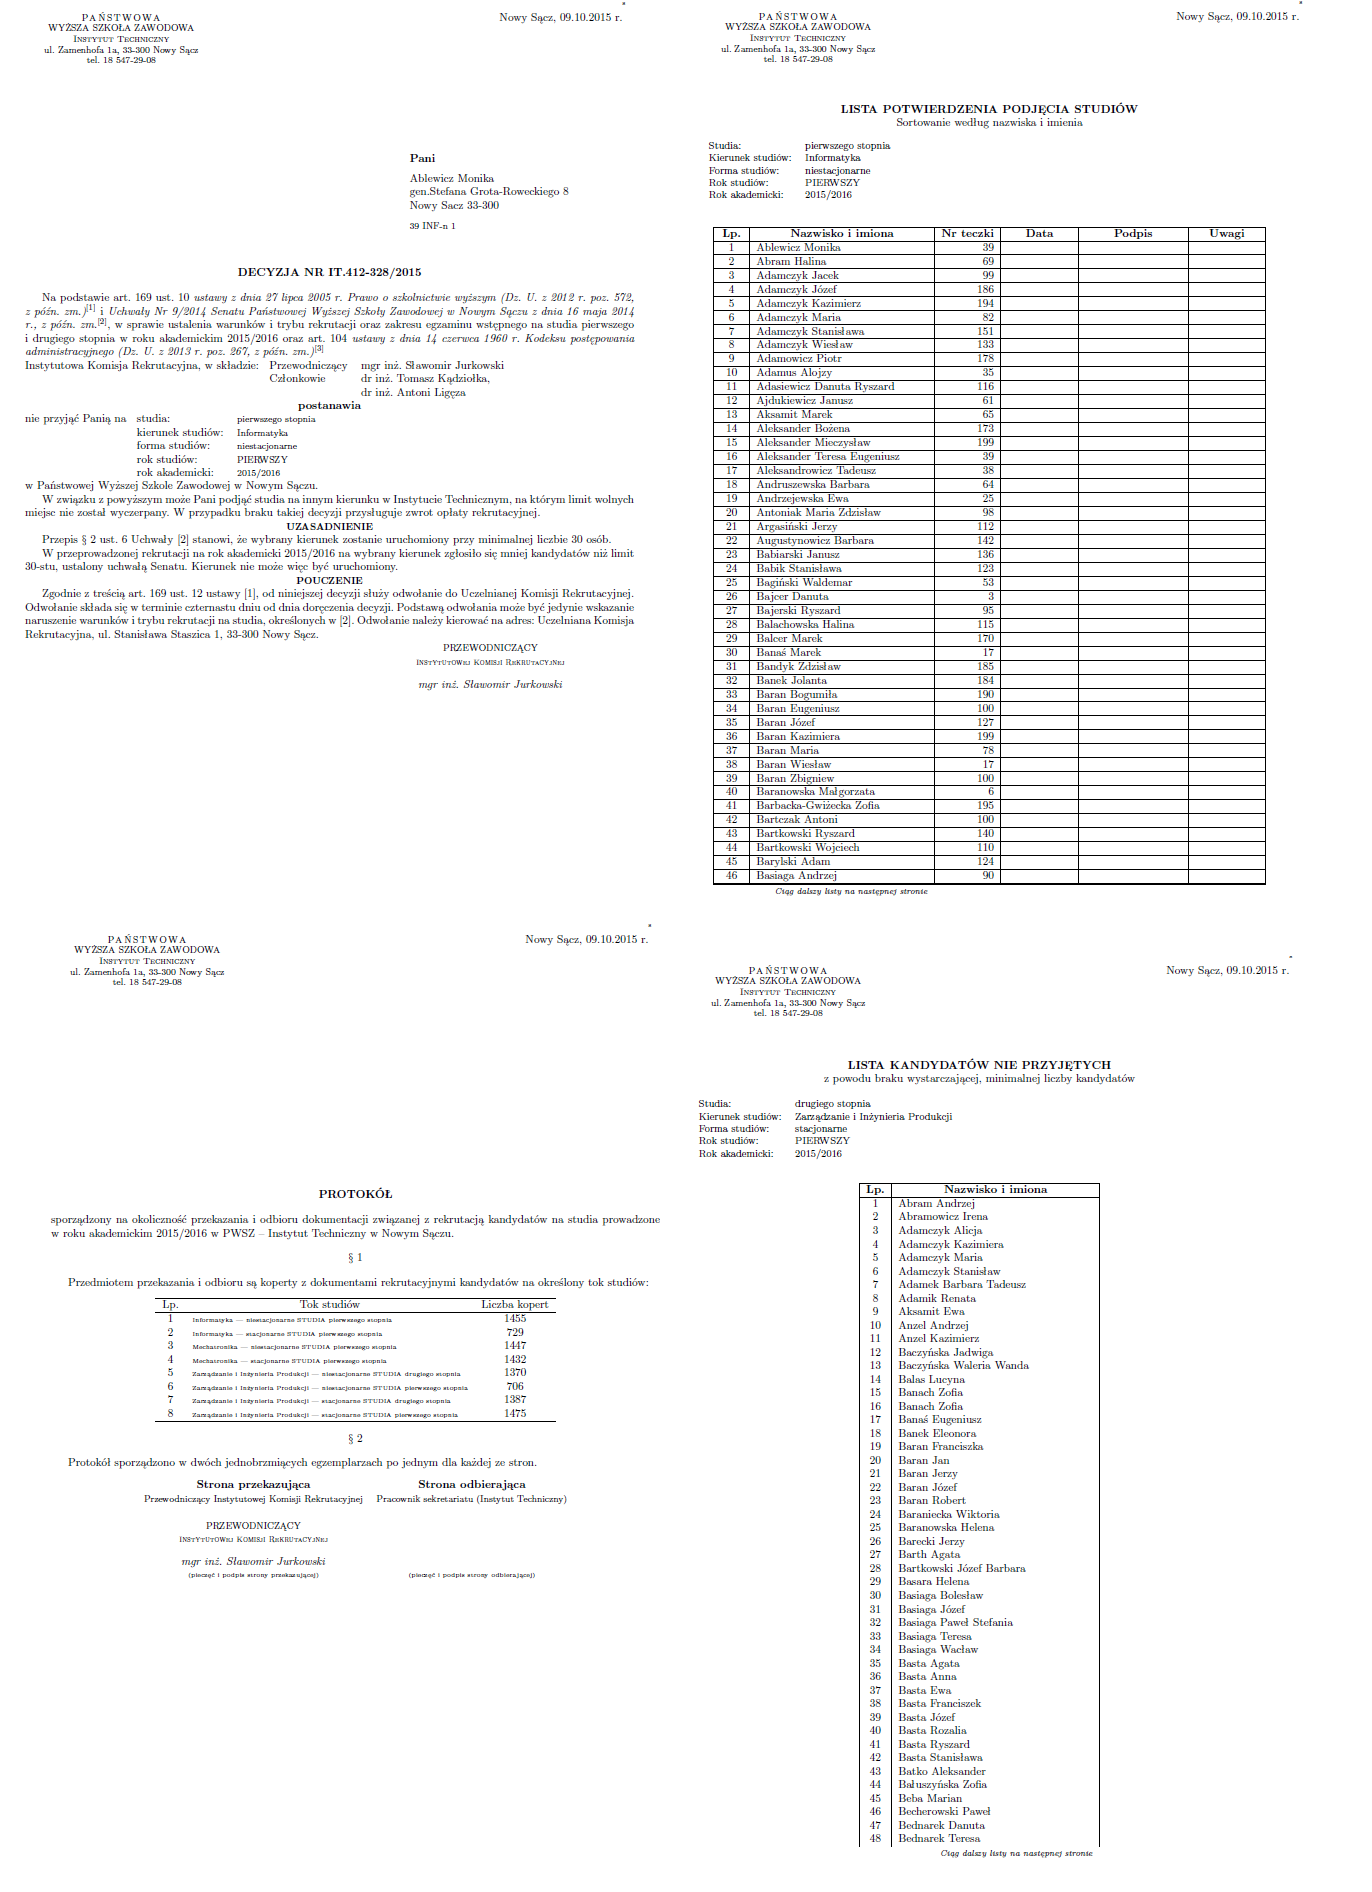
\includegraphics[width=0.8\textwidth]{rys/testy/wynik.png}
    \caption{Przykładowe strony wygenerowanych dokumentów z  testu }
    \label{fig:test}
\end{figure}
\section{Wnioski}
Po udanym przeprowadzeniu testu można stwierdzić, że tak przygotowana paczka systemu raportów zawierająca wszystkie rzeczy do przeprowadzenia rekrutacji, spełnia w pełnym zakresie wymagania postawione w założeniach pracy. Cały katalog roboczy systemu po spakowaniu zajmuje około 50 megabajtów i po rozpakowaniu około 100 megabajtów co oznacza, że przy dzisiejszych nośnikach danych nie będzie problemu z przeniesieniem systemu. Dodatkowo paczka zaraz po rozpakowaniu na systemie Windows jest gotowa do pracy i wymaga jedynie zainstalowanego środowiska uruchomieniowego JAVA 1.8. Cały system tworzenia raportów znajduje się w załączniku 3.



\appendix

% tutaj załączniki

%\chapter*{Bibliografia}
\nocite{*}
\bibliographystyle{plplain}
%\bibliographystylebk{plplain}
%\bibliographystylest{plplain}
%\bibliographystyledoc{plplain}
% \bibliographystyleweb{plplain}
%\bibliographybk{BIB/books}
%\bibliographyst{BIB/books}
%\bibliographydoc{BIB/books}
% \bibliographyweb{BIB/books}

% \bibliography{bib/verificard,bib/jml,bib/daikon}
\bibliography{bib/daikon,bib/statistics,bib/other}

\end{document}

% ex: set tabstop=4 shiftwidth=4 softtabstop=4 noexpandtab fileformat=unix filetype=tex spelllang=pl,en spell:

